\chapter{Projekt modułu ekstrakcji podsumowań}

Kolejny rozdział dotyczy projektu nowego modułu z wykorzystaniem odpowiednich diagramów UML. Przedstawiono również jego umiejscowienie na tle całej architektury aplikacji, a także omówiono schematy baz danych. 


\section{Baza danych}

Omówiona w niniejszym podrozdziale baza danych była obecne w pierwotnej wersji aplikacji. Jest ona podstawowym elementem w pracy agenta i odpowiada za przechowywanie obserwacji.

Baza obserwacji jest punktem łączącym tę aplikację, odpowiadająca za przetwarzanie danych, z inną, której głównym zadaniem jest wypełnianie bazy obserwacjami pojedynczych obiektów, dokonując oglądu otoczenia odpowiednimi narzędziami percepcyjnymi. Stanowi źródło danych agenta.

Schemat bazy danych tworzony jest z wykorzystaniem typów obiektów opisanych w~pliku \textit{type\_def.xml}. Na jego podstawie definiowane są zapytania DDL (ang. \textit{Data Definition Language} – czyli język definicji danych) języka SQL. Powstają w ten sposób tabele (listing \ref{rys:baza}) dotyczące konkretnych typów obiektów. Każda tabela składa się ze znacznika czasu (\textit{timestamp}), numeru identyfikatora (\textit{id}) oraz zbiór cech atomowych, gdzie każda jest w osobnej kolumnie. W \ref{lis:ddl} przedstawiono przykładowe zapytanie tworzące taką tabele. Zgodnie z założeniami ze wcześniejszych rozdziałów cecha może przyjąć trzy stany -- w~przypadku tabeli SQL będzie to \textit{1} (obecna), \textit{0} (nieobecna) oraz \textit{NULL} (nieokreślona).

\begin{listing}
\begin{minted}{text} 
CREATE TABLE IF NOT EXISTS “11” (
	timestamp integer NOT NULL,
	id text NOT NULL,
	Round integer CHECK (Red IN (1,0)),
	Colorful integer CHECK (White IN (1,0))
);
\end{minted}
	\caption{Przykładowe zapytanie DDL dla tabeli typu obiektu} 
	\label{lis:ddl}
\end{listing}

\begin{figure}  
	\centering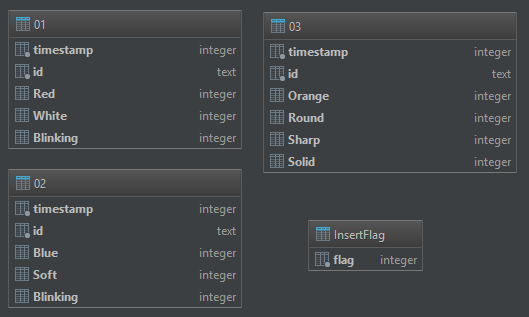
\includegraphics[width=.8\textwidth]{img/baza-schemat}
	\caption{Przykładowy schemat bazy danych \cite{raport}}
	\label{rys:baza}
\end{figure}

Istotnym elementem bazy jest tabela \textit{InsertFlag} widoczna na rysunku \ref{rys:baza}. Dzięki zaimplementowanemu wyzwalaczowi w bazie danych, który uruchamia się podczas dodawania nowych obserwacji do jednej z tabel, agent jest w stanie w prosty sposób sprawdzić, czy są w niej nowe rekordy. Wyzwalacz zmienia wartość flagi w tabeli \textit{InsertFlag}.

Obserwacje są pobierane poprzez oddzielną klasę dostępu do bazy - \textit{DatabaseAO}. Zdefiniowane w niej metody pozwalają na pobranie z bazy tylko nowych obserwacji. Na ich podstawie tworzone są epizody, które składają się na pamięć epizodyczną agenta.


\section{Architektura aplikacji bazowej}

Aplikacja agenta ma charakter złożonego systemu zbudowanego ze ściśle współpracujących modułów. Starano się zachować odpowiedni poziom elastyczności, który pozwoliłby na łatwe modyfikacje aplikacji. Główne moduły przedstawione są na rysunku \ref{rys:moduly}, a są to: moduł rdzenia agenta (odpowiada za realizację cyklu życia), moduł pamięci epizodycznej (odpowiada za przetwarzanie obserwacji i zarządzanie epizodami), moduł gruntowania (odpowiada za realizację procesu gruntowania wiedzy oraz zarządzanie pamięcią semantyczną -- holonami), moduł konwersacji (odpowiada za komunikację z użytkownikiem) oraz moduł symulacji (odpowiada za uruchamianie przygotowanych scenariuszy). Są to tylko najbardziej ogólne moduły, które dzielą się dodatkowo na wiele podmodułów. Oprócz tego w aplikacji zdefiniowane są też komponenty bardziej techniczne -- np.\ odpowiedzialne za wczytywanie plików konfiguracyjnych, czy utrzymywanie połączenia z bazą danych. Najbardziej istotne w kontekście tej pracy są moduły rdzenia agenta, pamięci epizodycznej i gruntowania. 

\begin{figure}  
	\centering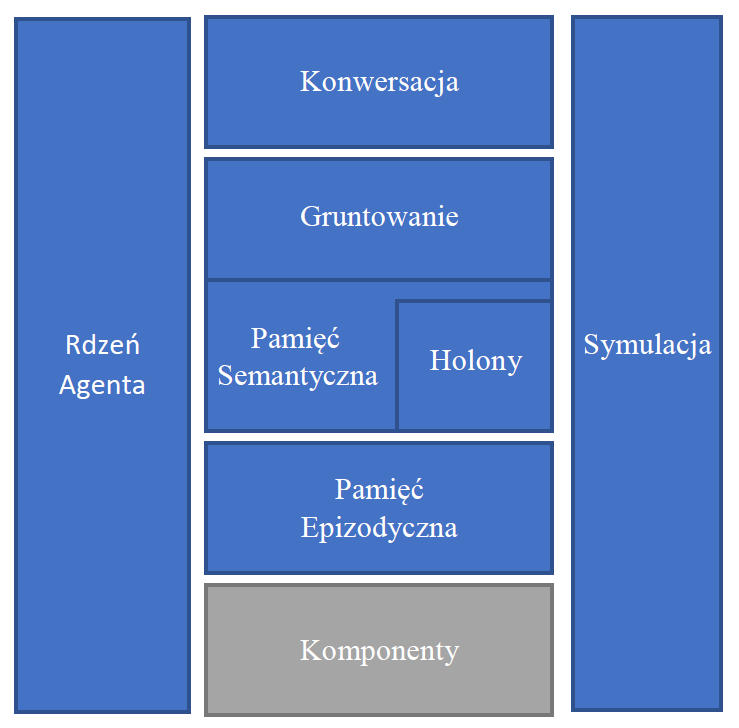
\includegraphics[width=.6\textwidth]{img/moduly}
	\caption{Modułowa architektura aplikacji agenta (na podstawie \cite{raport})}
	\label{rys:moduly}
\end{figure}

Podstawowym modułem systemu jest rdzeń agenta. Odpowiedzialny jest za synchronizację wykonywania poszczególnych procesów zachodzących w systemie. Wspomaga przetwarzanie obserwacji, ekstrakcje podsumowań wiedzy, odbieranie pytań i przekazywanie odpowiedzi do użytkownika, itp. Oprócz tego steruje cyklem życia agenta.

Moduł pamięci epizodycznej zarządza epizodami, czyli reprezentacją empiryczną wiedzy agenta. Jego zadaniem jest przetwarzanie obserwacji, zachowywanie właściwych struktur w kwestii typów obiektów oraz dystrybucja wiedzy z odpowiednich epizodów do innych modułów aplikacji.

Moduł gruntowania jest w kontekście tej pracy najbardziej istotny, gdyż to w jego obrębie zdefiniowany jest moduł ekstrakcji podsumowań danych, inaczej zarządzania pamięcią semantyczną. Realizuje przetwarzanie epizodów w celu uzyskania ilościowych (liczbowych) podsumowań wiedzy w postaci holonów. Zarządza, aktualizuje i przeszukuje holony.

Dalej opisano zmiany względem oryginalnej aplikacji.

\section{Struktura nowego modułu}

Na podstawie określonych wcześniej wymagań stworzono projekt nowego modułu ekstrakcji podsumowań danych. Oprócz samego modułu potrzebne będą również zmiany w cyklu życia agenta. Dodatkowo wymagane są niewielkie zmiany w dystrybucji wiedzy (epizodów) do tworzenia i aktualizowania holonów. 

Największym wyzwaniem jest proces aktualizacji holonów. Pierwotnie realizowana aplikacja nie zakładała w ogóle takiej możliwości -- holony za każdym razem były budowane od nowa. Przez to wymagana była całkowita przebudowa modułu ekstrakcji podsumowań danych.

Istotną zmianą względem poprzedniej implementacji jest tak zwana retrospektywna moc zbioru (ang. \textit{retrospective cardinality}). Jest to zmienna, w której przechowywana jest całkowita liczność wszystkich dotychczasowych zbiorów gruntujących. Umożliwia to aktualizacje przekonań (podsumowań), wyłącznie na podstawie danych z nowych obserwacji. Zgodnie z tymi założeniami zaprojektowano nowy moduł, który widać na rysunku \ref{rys:diagram-klas}.

\begin{figure}  
	\centering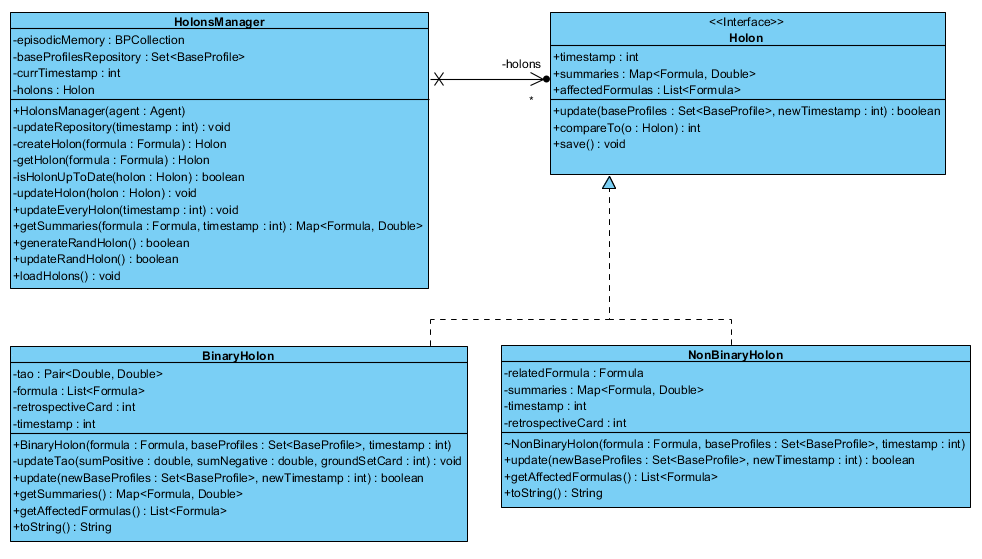
\includegraphics[width=\textwidth]{img/diagram-klas}
	\caption{Diagram klas nowego modułu ekstrakcji podsumowań danych}
	\label{rys:diagram-klas}
\end{figure}

W nowym module zastosowany interfejs \textit{Holon}, dzięki któremu zachowano duże podobieństwo między klasami dotyczącymi holonów prostych (\textit{BinaryHolon}) i holonów złożonych (\textit{NonBinaryHolon}) oraz zgodne interfejsy, czyli metody publiczne, używane przez obiekty innych klas. Zawierają metody pozwalające na ich aktualizowanie, porównywanie, a także zapisywanie z użyciem serializacji (\textit{save()}).

Opracowano również klasę o nazwie \textit{HolonManager}, która zarządza holonami i przechowuje ich kolekcję. Odpowiada ona za wszystkie możliwe działania związane z holonami: tworzenie, aktualizacja, zwracanie podsumowań. Dodatkowo pozwala na wczytywanie holonów, zapisanych przed ostatnim wyłączeniem agent, do pamięci (\textit{loadHolons()}).

W celu spełnienia wszystkich wymagań potrzebne są też modyfikacje w cyklu życia agenta. Klasa \textit{HolonManager} zawiera odpowiednie metody pozwalające na generowanie nowych, losowych holonów (\textit{generateRandHolon()}) oraz aktualizowanie ich w trakcie bezczynności (\textit{updateRandHolon()}). Nowy cykl życia agenta przedstawiono na rysunku~\ref{rys:cykl}. 

\begin{figure}  
	\centering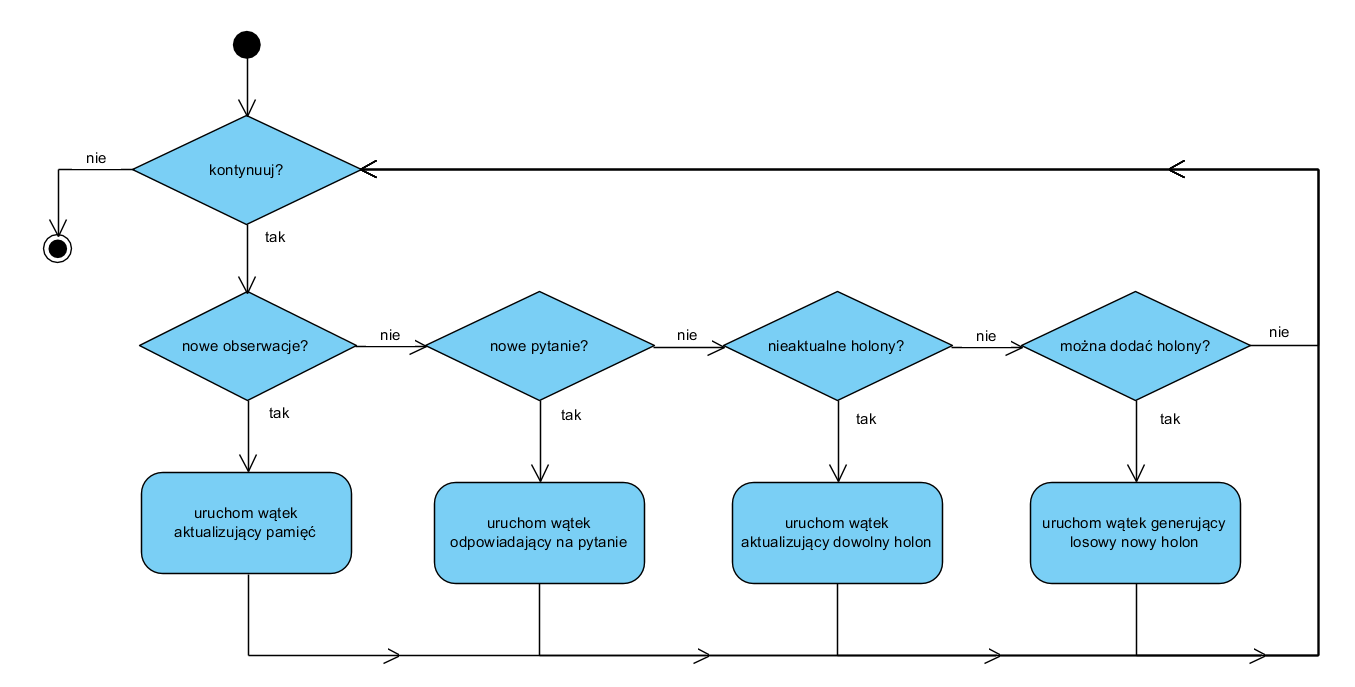
\includegraphics[width=\textwidth]{img/cykl}
	\caption{Diagram aktywności zmodyfikowanego cyklu życia agenta}
	\label{rys:cykl}
\end{figure}

Należy zwrócić uwagę na to, że zarządzanie wątkami w systemie zostało zrealizowane w taki sposób, żeby jednocześnie mógł być uruchomiony tylko jeden wątek. Wykorzystano w tym celu tak zwany semafor (więcej informacji o zarządzaniu wątkami można znaleźć w~\cite{java}). Jeśli zasób jest zajęty (jest aktywny wątek), to inne wątki są zmuszone czekać, aż się zwolni.

Cykl życia agenta pozwala na uzupełnienie agenta o dodatkowe funkcjonalności, które mogą być autonomicznie wykonywane w trakcie jego działania. W sytuacji gdy agent usłyszy pytanie może samodzielnie zdecydować czy chce i może w danym czasie na nie zareagować. Taka reakcja traktowana jest jako niezależne zachowanie typu \textit{one-shot behaviour}, czyli zadanie uruchamiane za każdym razem, gdy jest potrzebne. Takie podejście inspirowane jest mechanizmami zachowań agenta przedstawionymi w \cite{jade}. 



